%%%%%%%%%%%%%%%%%%%%%%%%%%%%%%%%%%%%%%%%%%%%%%%%%%%%%%%%%%%%%%%%%%%%%%%%%%%%%%%%%%%%%%%%%%%
%%
%% The updated version of this document should be downloaded from
%%      https://github.com/jp-um/university_of_malta_LaTeX_dissertation_template
%%
%% In case of any difficulties please contact Dr JP Ebejer on jean.p.ebejer@um.edu.mt
%%
%%%%%%%%%%%%%%%%%%%%%%%%%%%%%%%%%%%%%%%%%%%%%%%%%%%%%%%%%%%%%%%%%%%%%%%%%%%%%%%%%%%%%%%%%%%

%% Before you embark on this quest you should probably read some of:
%% Deadly sins - http://ctan.mirror.garr.it/mirrors/CTAN/info/l2tabu/english/l2tabuen.pdf
%% Writing a thesis in LaTeX - http://tug.org/pracjourn/2008-1/mori/mori.pdf

\RequirePackage[l2tabu, orthodox]{nag} % tells you of any bad LaTeX usage
                                       % must be first thing in class (with the exception of comments)

%% There is one option you should define; oneside or twoside
%% Use twoside for your viva docs (examiners hate long docs they need to carry around)
%% and oneside for the final thing you submit to the library.  Note that margins will
%% change accordingly

\documentclass[twoside]{um}  % custom University of Malta project/dissertation/thesis 


%% **************** (Your) Packages (Start) ******************

% \listfiles % uncomment this to know which packages you are using
              % the list of packages will be in the bottom of the .log file

%% Note that packges may already be loaded from the um (and memoir) classes.
%% Do not add your packages to the template, but rather add them here.

\usepackage{blindtext} %% for some dummy text, remove in your writeup
\usepackage{coffee4}    %% for some fun

%% ***************** (Your) Packages (End) *******************


%% **************** (Your) Data (Start) ******************

\title{Fiber Optic}  % use \\ here otherwise you get a justified title
                                                    % note capitalization of the title (only common 
                                                    % words in lower case)
\tagline{Stock Management System}                     % tag line
\author{Khalil SLEIMI}                           % your name
\authorID{12196/A}                           % your University Identifier
\supervisor{Mr Moez BOUTERAA}                             % your supervisor(s) name - no . in Dr
\cosupervisor{Mr Alaa LAABIDI}                               % your cosupervisor(s) name - no . in Dr ** OPTIONAL ** 
                                                    % simply comment out the above line if absent
\department{Department of Information and Communication Technologies}                  % your department (e.g. Artifical Intelligence)
\faculty{National Engineering School of Tunis}                      % your faculty (e.g. ICT)
\degree{Software Engineering}                      % the degree you are reading
                                                    % note the \ after the dot, so not to consider it a fullstop
\doctype{Internship Report}                              % the type of document (fyp, dissertation, thesis)
\degreedate{From 06 Jul. To 07 Aou. 2019}                        % when did you submit -- officially after your corrections !
%%\subjectcode{ICS5200}                               % the study unit-code (currently not used)

%% ***************** (Your) Data (End) *******************


%% ******** (Your) Document Settings (Start) *************

% You should have an images directory in every chapX subdir
% NOTE:  Trailing / for subdirs is required.
\graphicspath{{./images/}{./chap1/images/}}   % Paths where to look for images, if defined "images" must always be there as it holds the images in-use by the template.

\makeindex

%% ********* (Your) Document Settings (End) **************

% DOCTOR'S (JP) ORDERS: MAKE SURE TO READ MY TWO BLOG ENTRIES WITH
% CONTENT AND LaTeX TIPS FOR YOUR WRITE-UP.  THESE ARE BASED ON  
% EXAMINER'S FEEDBACK
%
% URLS:
% https://bitsilla.com/blog/2019/03/content-tips-for-your-dissertation-or-project-write-up/
% https://bitsilla.com/blog/2019/01/latex-tips-for-your-dissertation-or-project-write-up/

% end the preamble and start the document

\begin{document}
\frontmatter 
    \maketitle
    \begin{copyrightenv}
\end{copyrightenv}
       
    \begin{originality}
\end{originality}    
    %\begin{dedication}
%{\large{To The Avengers}}\\[5mm]
%You know, for saving the world.
%\end{dedication}

\begin{dedication}
{\large{Everything not saved will be lost.}}\\[5mm]
--Nintendo 'Quit Screen' message
\end{dedication}

%\begin{dedication}
%{\large{This report is for my Parents, who tried.}}\\[5mm]
%\end{dedication}        % include a dedication.tex file
    \begin{acknowledgements}
%\textbf{These are the acknowledgements.}%
 I'd like to take the time to acknowledge My Supervisor \textbf{Moez BOOTERAA} for all the help  he gave and the work inducive environment he provided. I'd also like to acknowledge my co-Supervisor \textbf{Alaa LAABIDI} for always being there for me to check my progress, helping  and all the encouragement and trust he puts in me. I'd also like to thank \textbf{My Sister} for her constant encouragement and help, but most importantly I'd like to thank \textbf{My Parents} for all their efforts raising me up and guaranteeing such an environment that allowed me to flourish into who I am Now. For all the Times they spent thinking and worrying about me, Thank you.\\Thank you all, I appreciate it, I'd also like to thank \textbf{ENIT} and all the \textbf{Teachers} and \textbf{Staff} for their insights: True Growth Comes from your own efforts, hard work and curiosity, the school can only give you a gentle glimpse at best.%\blindtext
\end{acknowledgements}   % include an acknowledgements.tex file
    %% For tips on how to write a great abstract, have a look at
%%	-	https://www.cdc.gov/stdconference/2018/How-to-Write-an-Abstract_v4.pdf (presentation, start here)
%%	-	https://users.ece.cmu.edu/~koopman/essays/abstract.html
%%	-	https://search.proquest.com/docview/1417403858
%%  - 	https://www.sciencedirect.com/science/article/pii/S037837821830402X

\begin{abstract}
%\textbf{This is the abstract.}%
	%This  internship  report stresseson  the  work  experience  I  have  gathered  as an  Intern in the --- department of Tunisie Telecom. from July 6, 2019 until Aout 7, 2019 (actually Aout 30, 2019).
  \textbf{Stock Management Programs} that are based on \textbf{Databases} can be a huge time savior, lowering the \textbf{time} it takes to find what you're looking for and minimizing the risk for \textbf{data inconsistencies} and \textbf{redundance} that are found among many alternatives like .xml files, also it can guarantee a \textbf{separation of concerns} through different \textbf{permissions}, and that in turn lowers the risk of users tinkering with things they are not allowed to.\\
In this report we talk about the \textbf{conception}, \textbf{design} and \textbf{realisation} of a Stock Management WebApp for Tunisie Telecom's Stock of fiber optics, with a separation of Permissions between what different User types can do.%\blindtext
\end{abstract}\if@openright\cleardoublepage\else\clearpage\fi
    \tableofcontents*\if@openright\cleardoublepage\else\clearpage\fi
    \listoffigures*\if@openright\cleardoublepage\else\clearpage\fi
    \listoftables*\if@openright\cleardoublepage\else\clearpage\fi
    %% will only print what is used ... useful.
%% also acronyms are clickable, which is awesome

\chapter*{List of Abbreviations}
\markboth{List of Abbreviations}{List of Abbreviations}
               
\begin{acronym}\itemsep-20pt\parsep-20pt %% if you remove these spacing params this list becomes huge!
\acro{DTC}{Digital Transmission Center}
\acro{TT}{Tunisie Telecom}

% \acro{CDMA}{Code Division Multiple Access}
% \acro{GSM}{Global System for Mobile communication}
% \acro{NAD+}[NAD\textsuperscript{+}]{Nicotinamide Adenine Dinucleotide}
% \acro{NUA}{Not Used Acronym}
% \acro{TDMA}{Time Division Multiple Access}
% \acro{UA}{Used Acronym}
% \acro{lox}[\ensuremath{LOX}]{Liquid Oxygen}
% \acro{lh2}[\ensuremath{LH_2}]{Liquid Hydrogen}
% \acro{IC}{Integrated Circuit}
% \acro{BUT}{Block Under Test}
% \acrodefplural{BUT}{Blocks Under Test}    
\end{acronym}
\if@openright\cleardoublepage\else\clearpage\fi

%% Note: always use \input as you cannot nest \includes (amongst other things)
\pagestyle{umpage}
\mainmatter 
    \chapter{Introduction}
\label{chap:intro}
\textbf{In this section I will explain and summarize what my internship and intership reports were all about and give a brief outline for the following chapters.}
\section{Motivation} % why is this a non trivial problem
	
	As part of my Computer Science Curriculum in the National Engineering School of Tunis, I wanted to complete my internship in a company that is in line with my professional orientation. I did not choose a Telecommunications Company because I wanted to switch to the field of Telecommunications afterwards, but because the mission that was proposed to me was consistent with my professional goals. \\  

	Indeed, my primary mission was to observe the environment and interaction of Tunisie Telecom's employees and their discipline and hard work, I also discovered several new tools and techniques that were above me, I also learned of several devices and techniques employed by Tunisie Telecom to guarantee their Networks are top notch, it was a great opportunity for me to actually be in such an environment, which gave me more courage as a student to see myself becoming a software engineer. \\
	
	In a second time, I had to design a Web Platform, which is accessible locally. Its role is to enable all Tunisie Telecom staff of Creating, Storing, Updating and Deleting different entries of a Fiber Optics stock management program according to their User Type, putting as a priority the simplicity and efficiency of the Web Platform.\\

	Finally,  I'm very satisfied of this internship because it introduced me to a lot of new concepts like HTML, CSS, BootStrap, PHP, MySQL, LAMP stack, Linux and even Git Version Control Systems in a domain that I love. And also allowed me to highlight my skills aquired during my Software Engineering year of studies. \\ 

The place where I did the Internship is shown in Figure~\ref{fig:test1}.
\begin{figure}[ht!] % supposedly places it here ...
  \centering
  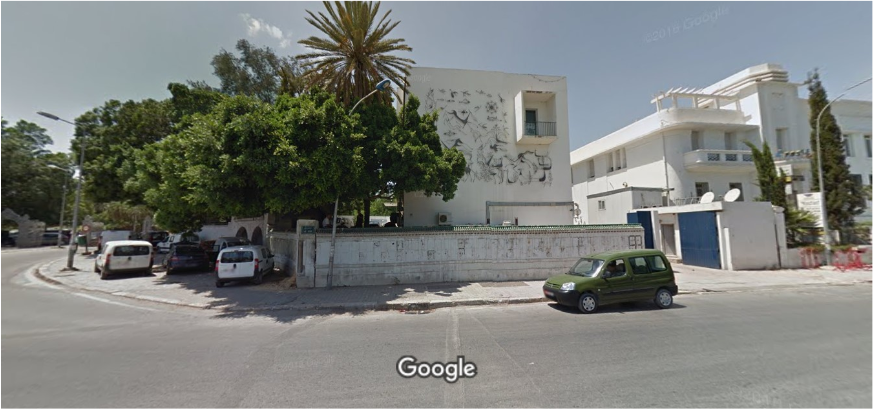
\includegraphics[width=0.6\linewidth]{test_image_goku}
  \caption[Where I Did the Internship]{Tunisie Telecom \index{Goku il-king}}%
  \label{fig:test1}
\end{figure}

	This is an Image from Google Maps of the Digital Transmission Center (Centre de Transmission Numérique - CTN) of Tunisie Telecom based in Place Pasteur, Belvedere, hereafter noted DTC. Where I did my Internship.

% \textbf{Note that you may have multiple \texttt{{\textbackslash}include} statements here, e.g.\ one for each subsection.}\cofeBm{0.7}{1}{0}{3cm}{-1cm}

\section{Aims and Objectives - Outline} 

	Besides this Chapter~\autoref{chap:intro} and the Conclusion~\autoref{chap:conc}. There are two main chapters:
	\begin{itemize}
	\item In Chapter~\autoref{chap:org},I will Introduce Tunisie Telecom DTC Belvedere, the company's history and its field of Telecommunications and the things I saw there, as well as the Data Unit (Unité Data) branch, that is responsible for dealing with big companies and clients in which I worked.
	\item In Chapter~\autoref{chap:app}, I will Introduce the Problem that we faced in Tunisie Telecom alongside the Solution I came up with, It's analysis, conception and realisation alongside the tools I learned throughout the way.
	%What's my aims and objectives??

	\end{itemize}
% \blindtext

% \begin{table*}\centering
% \ra{1.3}
% \begin{tabular}{@{}rrrrcrrr@{}}\toprule
% & \multicolumn{3}{c}{$w = 8$} & \phantom{abc}& \multicolumn{3}{c}{$w = 16$} \\
% \cmidrule{2-4} \cmidrule{6-8} 
% & $t=0$ & $t=1$ & $t=2$ && $t=0$ & $t=1$ & $t=2$\\ \midrule
% $dir=1$\\
% $c$ & 0.0790 & 0.1692 & 0.2945 && 0.3670 & 0.7187 & 3.1815\\
% $c$ & -0.8651& 50.0476& 5.9384&& -9.0714& 297.0923& 46.2143\\
% $c$ & 124.2756& -50.9612& -14.2721&& 128.2265& -630.5455& -381.0930\\
% $dir=0$\\
% $c$ & 0.0357& 1.2473& 0.2119&& 0.3593& -0.2755& 2.1764\\
% $c$ & -17.9048& -37.1111& 8.8591&& -30.7381& -9.5952& -3.0000\\
% $c$ & 105.5518& 232.1160& -94.7351&& 100.2497& 141.2778& -259.7326\\
% \bottomrule
% \end{tabular}
% \caption{A Beautiful and Complex Table}\label{tab:sometable}
% \end{table*}

% A beautiful table is shown in Table~\ref{tab:sometable}, data from \citet{Ebejer2012} (when citing as part of text, otherwise \citep{Ebejer2012}).


% \blindtext

% % \begin{figure}[ht!] % supposedly places it here ...
% %   \centering
% %   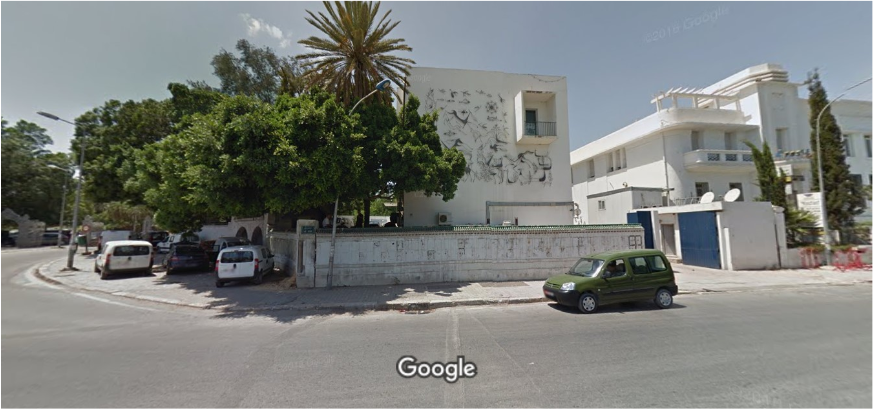
\includegraphics[width=0.6\linewidth]{test_image_goku}
% %   \caption[This is the short caption for List of Figures]{A test figure.  This caption is huge, but in the list of figures only the smaller version in the square brackets will appear.\index{Goku il-king}}
% %   \label{fig:test1}
% % \end{figure}



% \section{Proposed Solution} 

% \blindtext
% \blindtext

% \begin{figure}[!ht]
%     \centering
%     \subbottom[Goku]{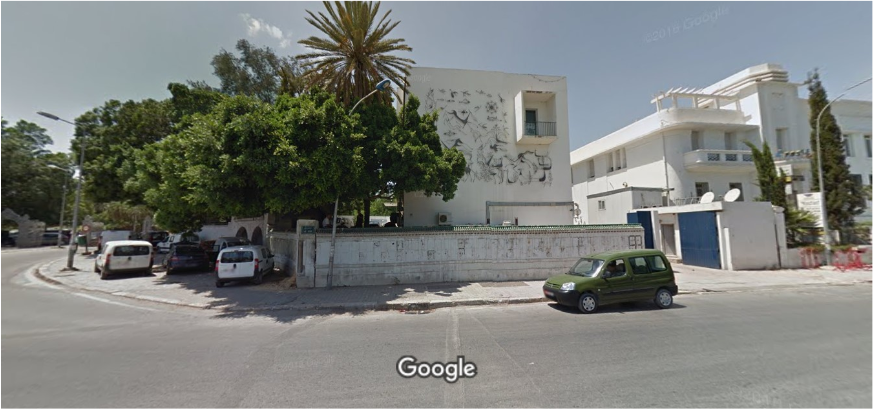
\includegraphics[width=0.3\textwidth]{test_image_goku}}\qquad
%     \subbottom[More Goku]{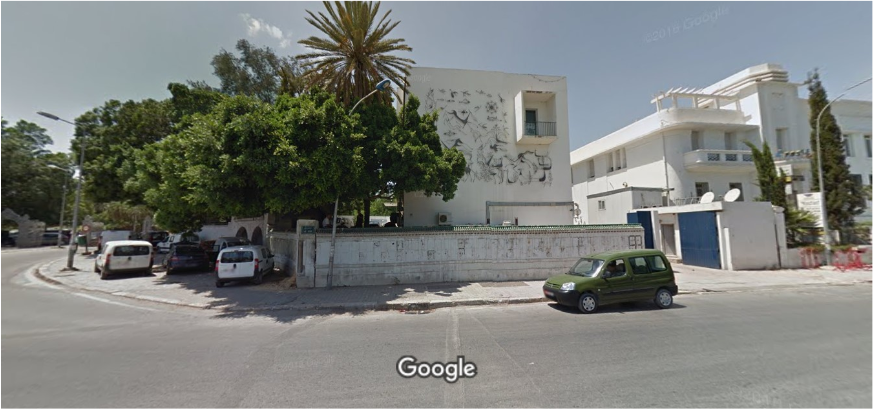
\includegraphics[width=0.3\textwidth]{test_image_goku}}%
%     \caption[Short Caption]{The same super saiyan. Two times.}        
%     \label{fig:test2}
% \end{figure}

% Two figures shown side by side are shown in Figure~\ref{fig:test2}.

% \subsection{Showing the Use of Acronyms}

% In the early nineties, \acs{GSM} was deployed in many European countries. \ac{GSM} offered for the first time international roaming for mobile subscribers. The \acs{GSM}’s use of \ac{TDMA} as its communication standard was debated at length. And every now and then there are big discussion whether \ac{CDMA} should have been chosen over \ac{TDMA}.

% If you want to know more about \acf{GSM}, \acf{TDMA}, \acf{CDMA} and other acronyms, just read a book about mobile communication. Just to mention it: There is another \ac{UA}, for testing.


% \section{Document Structure}

% \blindtext
 
    \chapter{Organization Overview} % Background \& Literature Overview
\label{chap:org}
\textbf{In this section we'll review Tunisie Telecom's History, Notable leaders, Its' business sector and the wide range of clients it offers its services to, as well as its' organizational hierarchy and the work environment I witnessed.  (i.e.\ in the following sections)}
\section{Introduction to Tunisie Telecom \& History} % Some Technique One
\index{Introduction to Tunisie Telecom \& History|(}%%Some Technique One

%\blindtext
\index{Introduction to Tunisie Telecom \& History!Introduction to TT}%%Some Sub-technique One%make it the subsection name
%\blindtext
\subsection{Introduction to TT}%Some Sub-sub-technique One
Tunisie Telecom is the brand name of the historical provider of telecommunication services in Tunisia. Its capital is 875 million euros and its transaction number, in 2004, amounted to 750 million euros.

Tunisie Telecom has more than 6 million fixed and mobile subscribers in Tunisia and abroad. It also plays an important role in improving the Internet's influence in Tunisia, which ultimately allowed it to have 140,000 subscribers by the end of April 2008.
\textbf{Comment: Find more recent data}

\index{Introduction to Tunisie Telecom \& History!History}%%Some Sub-sub-technique One%make it the subsection name to which you want to jump
%\blindtext
\subsection{History}
The law establishing the National Telecommunications Office, whose commercial name is Tunisie Télécom, was promulgated on 17 April 1995 and came into force on 1 January 1996.

Tunisie Télécom sets up, operates and markets the first GSM network in Mauritania (Mattel) from May 2000. It also enters into a technical cooperation agreement with Djibouti Telecom for the development of its telecommunications networks.

It became a public limited company at the end of 2002, it changes its legal status, by a decree of April 5, 2004, to become a limited company called "Tunisie Telecom". It is experiencing partial privatization in July 2006 with the entry into its capital, up to 35\%, of the Emirati consortium EIT (Emirates International Telecommunications).

From 2008, Tunisie Telecom offers the possibility to national bank card holders to feed the balance of their prepaid lines via ATMs of the Arab Tunisian Bank (Mobilink service).

On March 21, 2009, Tunisie Telecom launched a new brand, Elissa, with offers specifically designed for young people under 25; it becomes accessible to all without age limit as of March 10, 2012.

In the spring of 2011, following the Tunisian revolution, the company is shaken by a major social conflict between the representatives of the Tunisian General Labor Union (UGTT) and those of its UAE shareholder over the fate of some 60 contracts representing 3.5\% of the payroll; it is marked by strikes and sit-ins affecting the proper functioning of the operator. It ends with the end of these employment contracts, with the exception of ten contract holders retaining their positions.

In September 2012, Chief Executive Officer (CEO) Ali Ghodhbani retires and is replaced by Mokhtar Mnakri, former CEO of Alcatel's subsidiary.

In 2014, Salah Jarraya was appointed CEO to replace Mnakri, whose term was coming to an end.

In June of the same year, the employees started a social movement to obtain a salary increase and to claim the application of the agreements signed in February 2011. They gather around the UGTT and carry out many work stoppages until May they succeed in May 2015. Following these social movements and strikes, Jarraya resigns on July 2nd.

On August 12, Nizar Bouguila is appointed CEO.

On March 15, 2016, Tunisie Telecom launched its new visual identity called "Life is Emotions", with a new logo. In August, Tunisie Telecom finalizes the purchase of 65.4\% of the entire capital of GO (en).

Bouguila is replaced on September 19, 2017 by Mohamed Fadhel Kraiem. On November 7, Tunisie Telecom signed a five-year contract with the Ministry of Information Technologies and the Digital Economy to cover white areas with broadband telecommunications services.

On December 13, 2017, UAE investment fund Abraaj announced that it had signed an agreement the day before for the definitive purchase of EIT's 35\% stake. However, the bankruptcy of the fund cancels the operation.




%\blindtext

%\blindtext
\index{Introduction to Tunisie Telecom \& History|)}

\section{Global Leaders of Tunisie Telecom}%[Some Technique Two]{Some Technique Two with Super Long Title Which Will Overrun In Header}
\index{Global Leaders of Tunisie Telecom|(}%%Some Technique Two
%\blindtext[5]
Ali Ghodhbani - Mokhtar Mnakri - Salah Jarraya - Nizar Bouguila - Mohamed Fadhel Kraiem

%Imagine some colourful description on Some Technique Three\index{Some Technique Three}.

\index{Some Technique Two|)}

\section{Activities of Tunisie Telecom \& Clients}% Evaluation Criteria
This section should contain information on the metrics and background used to evaluate your work.
\section{Related Work}
\textbf{In this section you need to explain (and reference) similar work in literature}.  Make sure to:

\begin{itemize}
 \item Give a systematic overview of papers with related/similar work
 \item Highlight similarities/differences to your work (perhaps in the form of a table)
\end{itemize}

Note that this section may be sectioned based on the different aspects of your dissertation.  Some referenced text, as an example \citep{Arrighi2003, WithersMartinez2012, Ebejer2016}.

\section{Organizational Hierarchy}
The Organizational Hierarchy of Tunisie Telecom is shown in Figure~\ref{fig:tt1}.
%\begin{figure}[ht!] % supposedly places it here ...
%  \centering
%   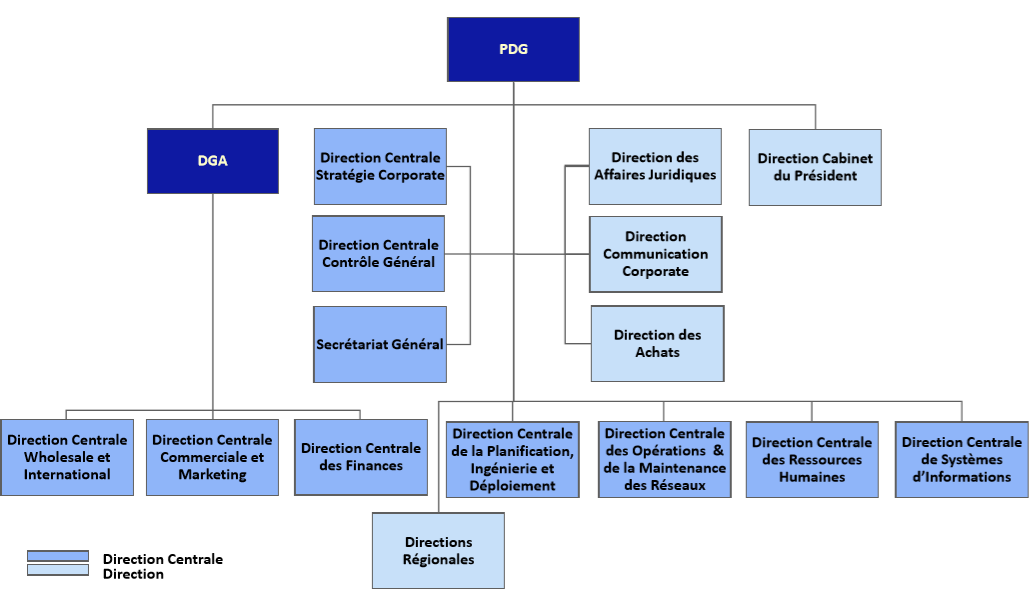
\includegraphics[width=0.6\linewidth]{TT_Hierarchy}
%  \caption[TT Hierarchy]{Tunisie Telecom \index{Goku il-king}}%
%  \label{fig:tt1}
%\end{figure}


% 	To be done later
% ⦁ Structure of the center:

% The belvedere telecommunication complex consists of several centers and services. Following this general presentation, we will move to the precise study of the CC (Switching Center) and the CTN (Digital Transmission Center) where we spent the month of internship.

% Figure 3: Center Structure
% ⦁ Line switching center:

% The CCL is a service that manages the maintenance of the switched network and the installation of transmission cables that connect the subscribers to the central office and the exchanges between them.
% ⦁ Switching Center:

% The Belvedere complex contains two switching exchanges intended to maintain the switching system; The ERICSSON Swedish AX system and the German EWSD system from Siemens. The center is responsible for all subscriber registration operations in the system as well as operations related to fixed telephony services such as prepaid, international calls or caller ID display.
% ⦁ Digital Transmission Center:

% The digital transmission center is one of the basic cells in the telecommunication network. It is the speaker of digital transmission media. In a future chapter of our report, we will take care of his presentation.



% 	This is an Image outlining the Organizational Hierarchy of Tunisie Telecom



\section{Work Environment}
\blindtext
    \chapter{The Stock Management Web Application} % Materials \& Methods
\label{chap:app}
\textbf{In this section I will represent what you did in the internship. The project as well as its Conception and design, the Tools Used and its Realisation.}

%\Blindtext
\section{Introduction}%Summary
	During the last two weeks of the internship, I was given the task to design and implement A stock management Web application for Tunisie Telecom's Stock of Fiber Optics, all for the benefits of a DBMS:  Efficiency, Reliability, Convenience, Safety, Multi-User storage of and access to massive amounts of persistent data.
\section{Tools Used}
	During my internship I used a number of tools including: \\
		- Kali Linux 2019.3 \& Elementary OS 5.0 Juno\\
		- LAMP 7.3.9 \\
		- Git 2.23.0 \& GitHub\\
		- Sublime Text 3.0 \\
		- MikTex 2.9.7100 \& TexWorks 0.6.3 \\
\section{Analysis \& Conception} % Database UML & class diagram & Use case
	In this Section I will Present a detailed analysis of the problem at hand and its proposed Conception.
\subsection{Analysis}
	We need to track each Fiber Optic Strand, to which Client it is reserved and on which optical fiber loop between Data Transmission Centers it is located. And give different roles to different Users.

\begin{figure}[ht!] % supposedly places it here ...
  \centering
  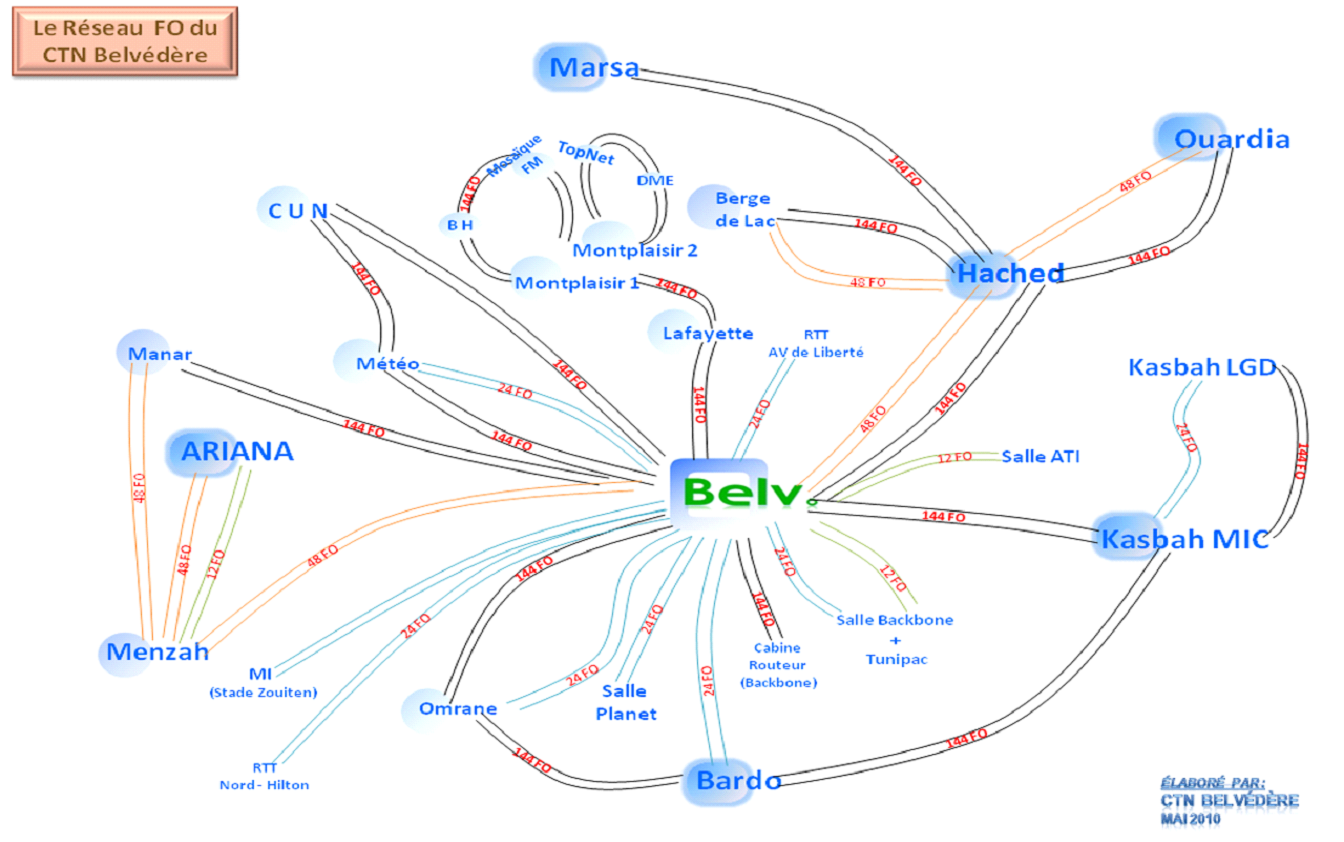
\includegraphics[width=\linewidth]{DTC_Belvedere}
  \caption[DTC Belvedere]{Optic Fibers Map}%\index{Goku il-king}}%
  \label{fig:OFMap}
\end{figure}
We definitely need this tool implemented as a DBMS because traditional .xls files doesn't provide redundancy control, nor does it give different users different profiles and roles, and we know that DBMS's provide all of that and so much more.
\begin{figure}[ht!] % supposedly places it here ...
  \centering
  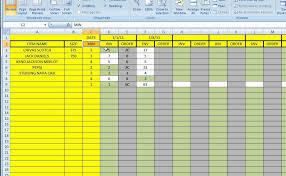
\includegraphics[width=\linewidth]{excel}
  \caption[Excel]{Optic Fibers Map}%\index{Goku il-king}}%
  \label{fig:HowTheyUsedToWork}
\end{figure}
The class diagram is shown in ~\ref{fig:DiagClass1}.
\subsection{Conception}
\begin{figure}[ht!] % supposedly places it here ...
  \centering
  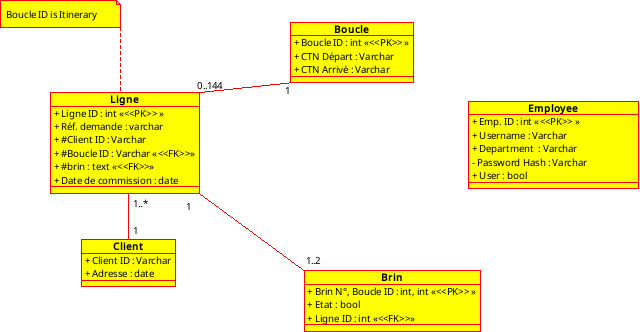
\includegraphics[width=\linewidth]{Class_Diagram}
  \caption[Class Diagram]{Conception}%\index{Goku il-king}}%
  \label{fig:DiagClass1}
\end{figure}
In the Class Diagram and in our project, all revolves around the FiberOptic Ligne, which belongs to a certain Client (company or individual and further details are out of the scope of this work), and is situated on a certain Circuit or 'Boucle' between DTC's, and also which Brin - Boucle pair are attributed to that Ligne along with the status. And then separately, there's an Employee with a status of Admin who has all the permissions on adding, modifying or even deleting Ligne, Client, Boucle, Brin and also other Employees. On the other hand a simple User can only create new Lignes for already existing Clients, on boucles that already exist.
There are 144 Brins per Boucle, and they can have either the status used or unused or under maintenance.
\section{Realisation}%Summary

%\blindtext
Here is a look at the Login screen, the DBMS will automatically recognize which role to grant the Employee. The password is a SHA-256 encrypted and saved in the DBMS.
\begin{figure}[ht!] % supposedly places it here ...
  \centering
  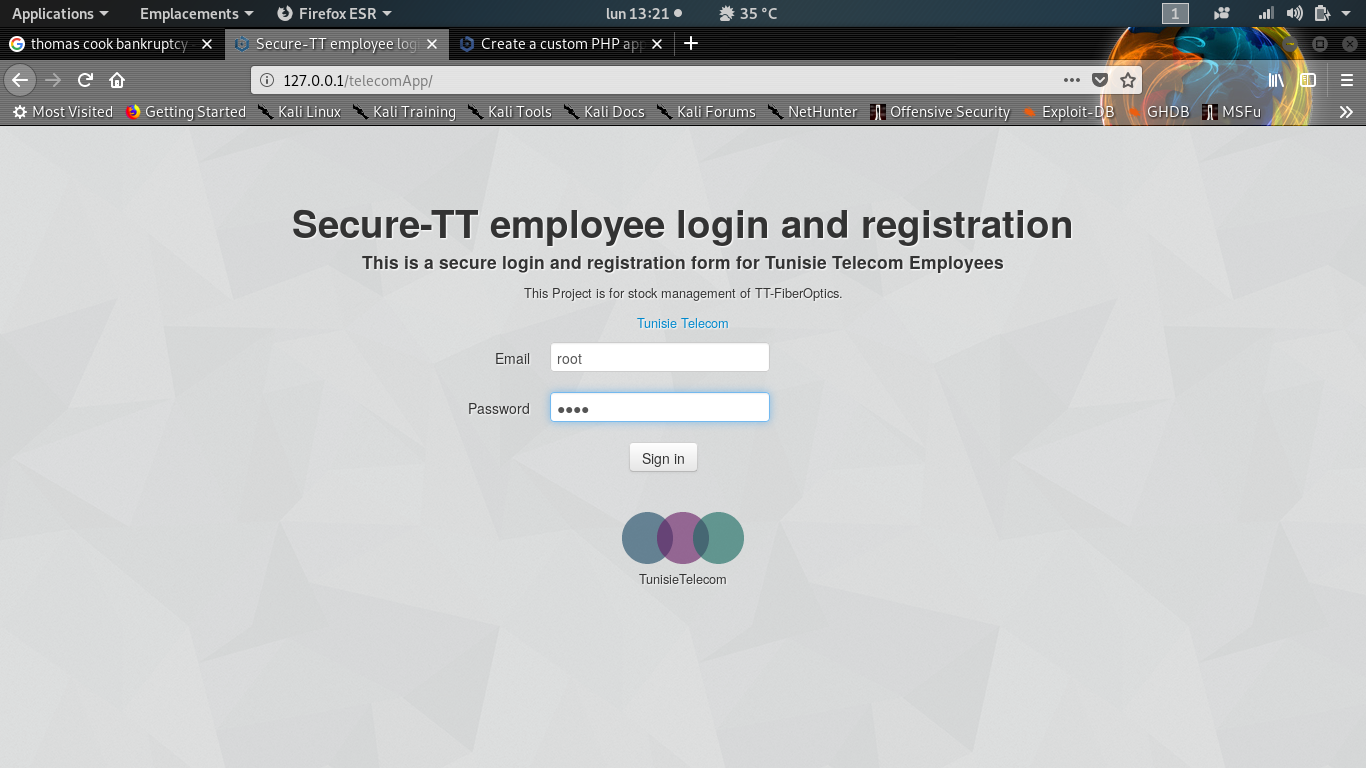
\includegraphics[width=\linewidth]{Login}
  \caption[Login]{Login Screen}%\index{Goku il-king}}%
  \label{fig:Login}
\end{figure}
A User - Employees Dashboard screen is shown below in Figure ~\ref{fig:UserTable}. As you can see, a User can only see things he's allowed to see, and can only modify these things exclusively.
\begin{figure}[ht!] % supposedly places it here ...
  \centering
  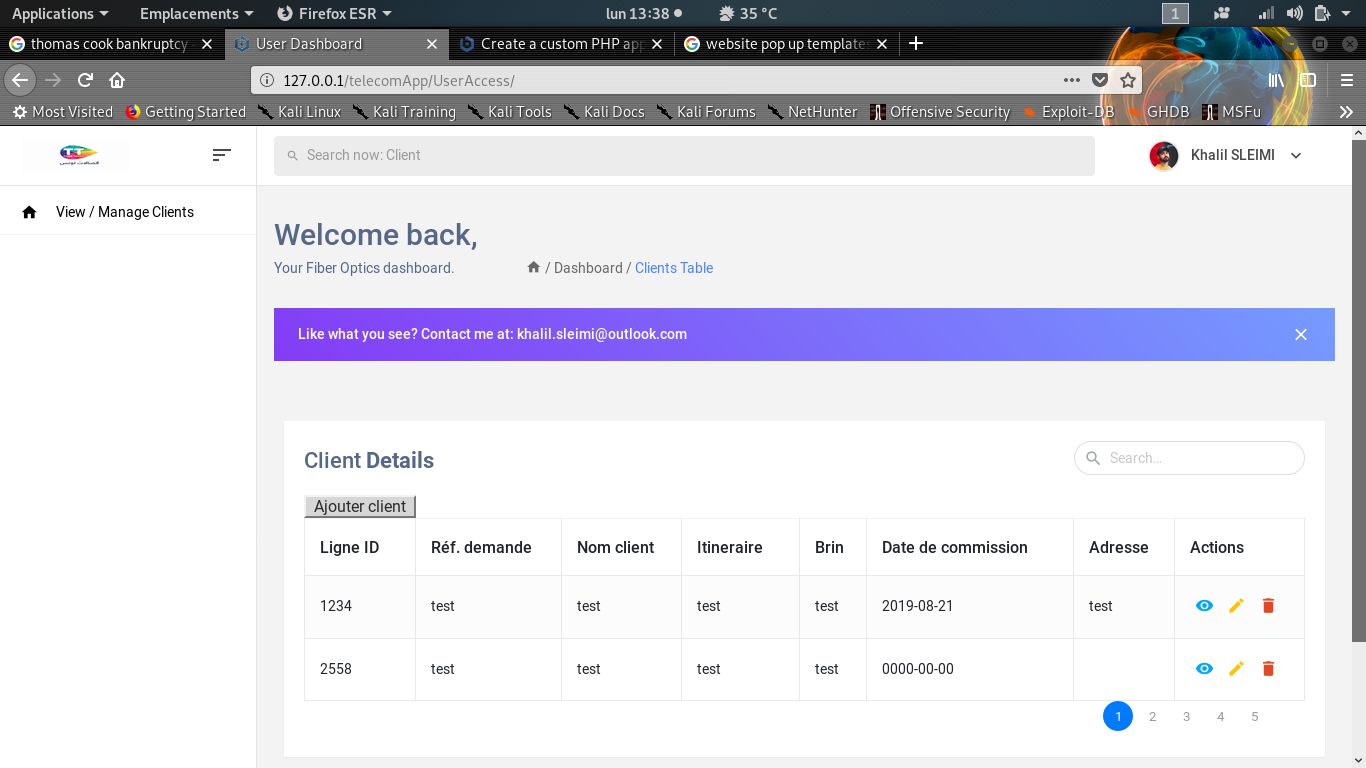
\includegraphics[width=\linewidth]{UserTableau}
  \caption[UserClientsTable]{ User Ligne}%\index{Goku il-king}}%
  \label{fig:UserTable}
\end{figure}
If the Login process recognizes the Employee as being the Admin, the Dashboard will be something like this, He have total control over everything, as is shown on the left, He can manage Clients, or what I presented in the Conception phase above as Ligne (I made the Implementation before the Conception, big mistake, I know), Employees, Boucles and Brins.
\begin{figure}[ht!] % supposedly places it here ...
  \centering
  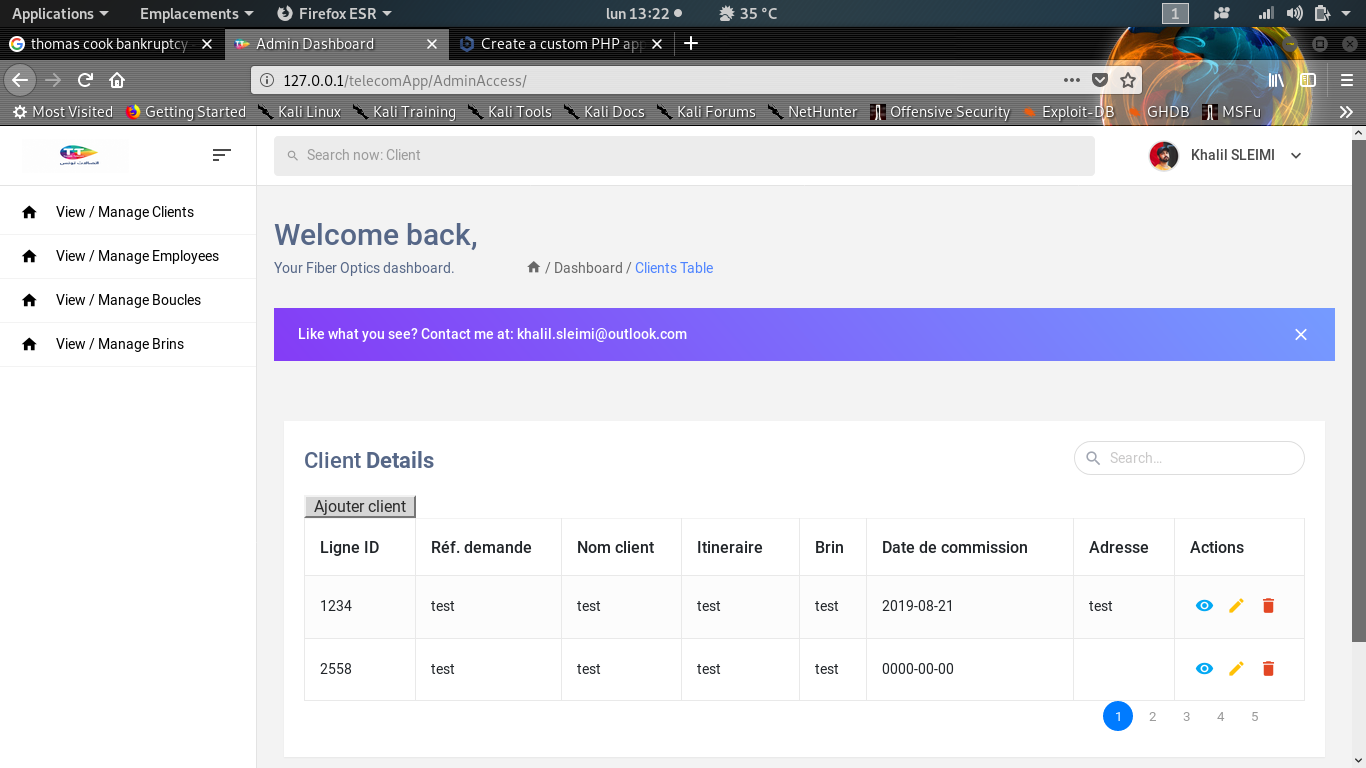
\includegraphics[width=\linewidth]{AdminTableau}
  \caption[AdminClientsTable]{Admin Ligne}%\index{Goku il-king}}%
  \label{fig:AdminClientsTable}
\end{figure}

In this Figure ~\ref{fig:AdminEmployeeTable}, the Admin is allowed to Add, remove or even modify any other Employee, If we'd want it to be some more professional, the Department field will be replaced by a Type field which is either "Admin" or "User". But this was done in less than a month from scratch, and also due to a HDD failure, I don't think I could've done any better - only if I had designed it from the get go and actively used github to back it up - and not forget "git add *" everytime I add some new file.
\begin{figure}[ht!] % supposedly places it here ...
  \centering
  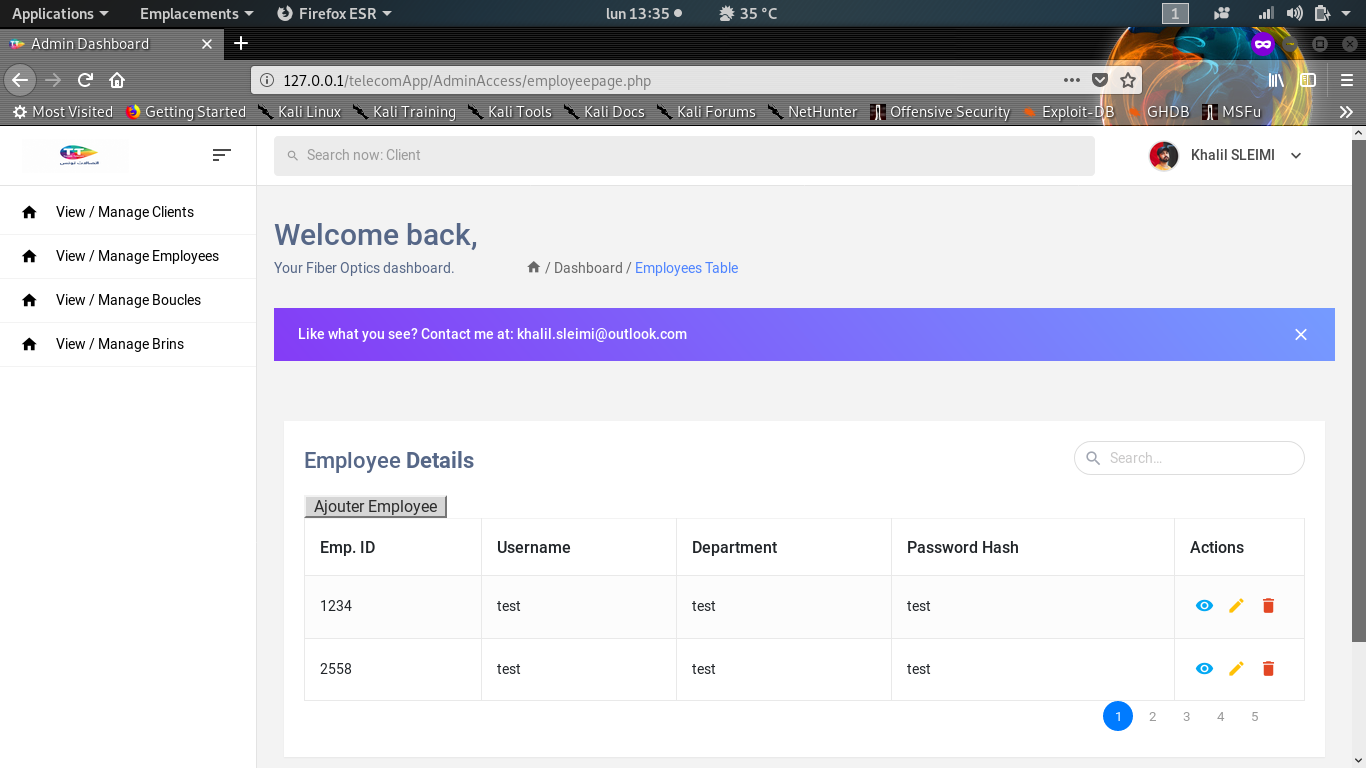
\includegraphics[width=\linewidth]{AdminEmployeeTableau}
  \caption[AdminEmployeeTable]{Admin Employee}%\index{Goku il-king}}%
  \label{fig:AdminEmployeeTable}
\end{figure}

Now, every Ligne is based on a certain Fiber Optic Boucle. This Menu allows the Admin to Manage these Boucles.
\begin{figure}[ht!] % supposedly places it here ...
  \centering
  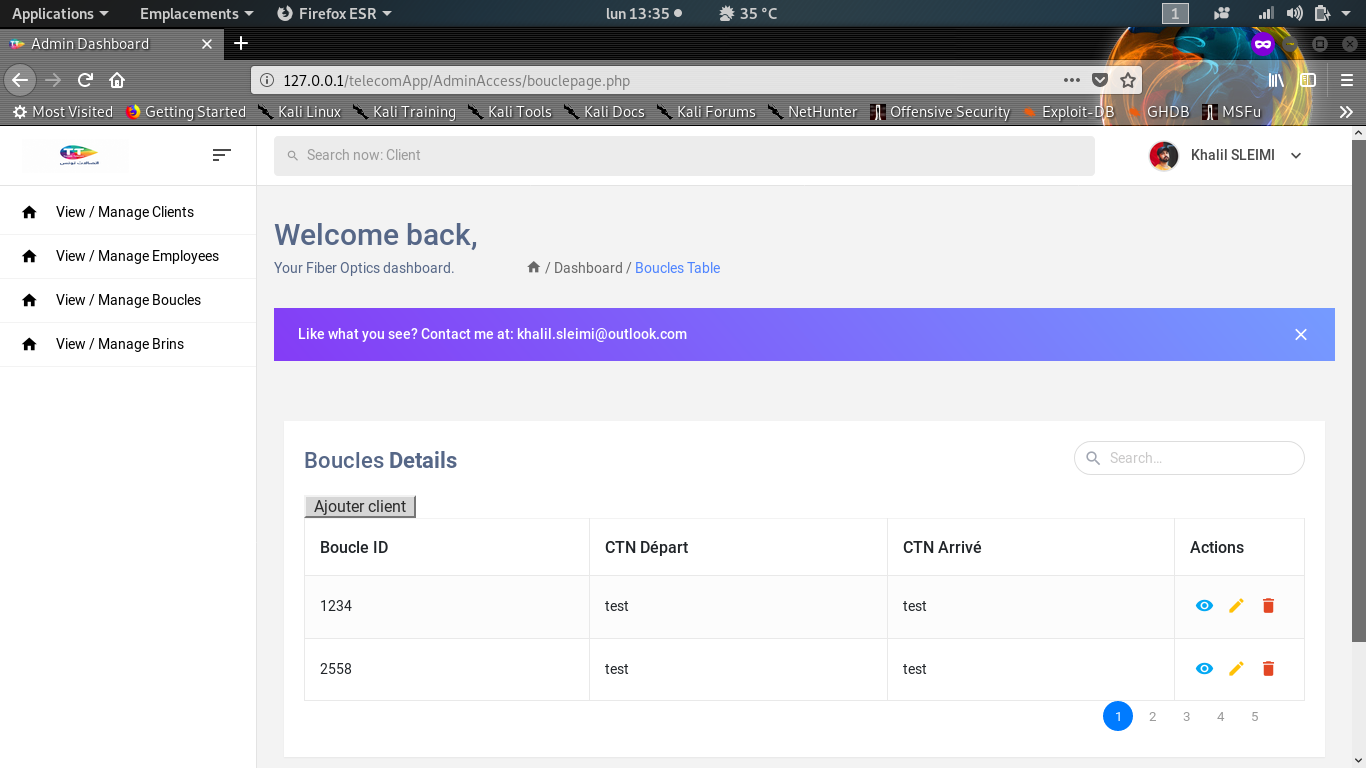
\includegraphics[width=\linewidth]{AdminBouclesTableau}
  \caption[AdminBouclesTable]{Admin Boucles}%\index{Goku il-king}}%
  \label{fig:AdminBouclesTable}
\end{figure}

% \begin{figure}[ht!] % supposedly places it here ...
%   \centering
%   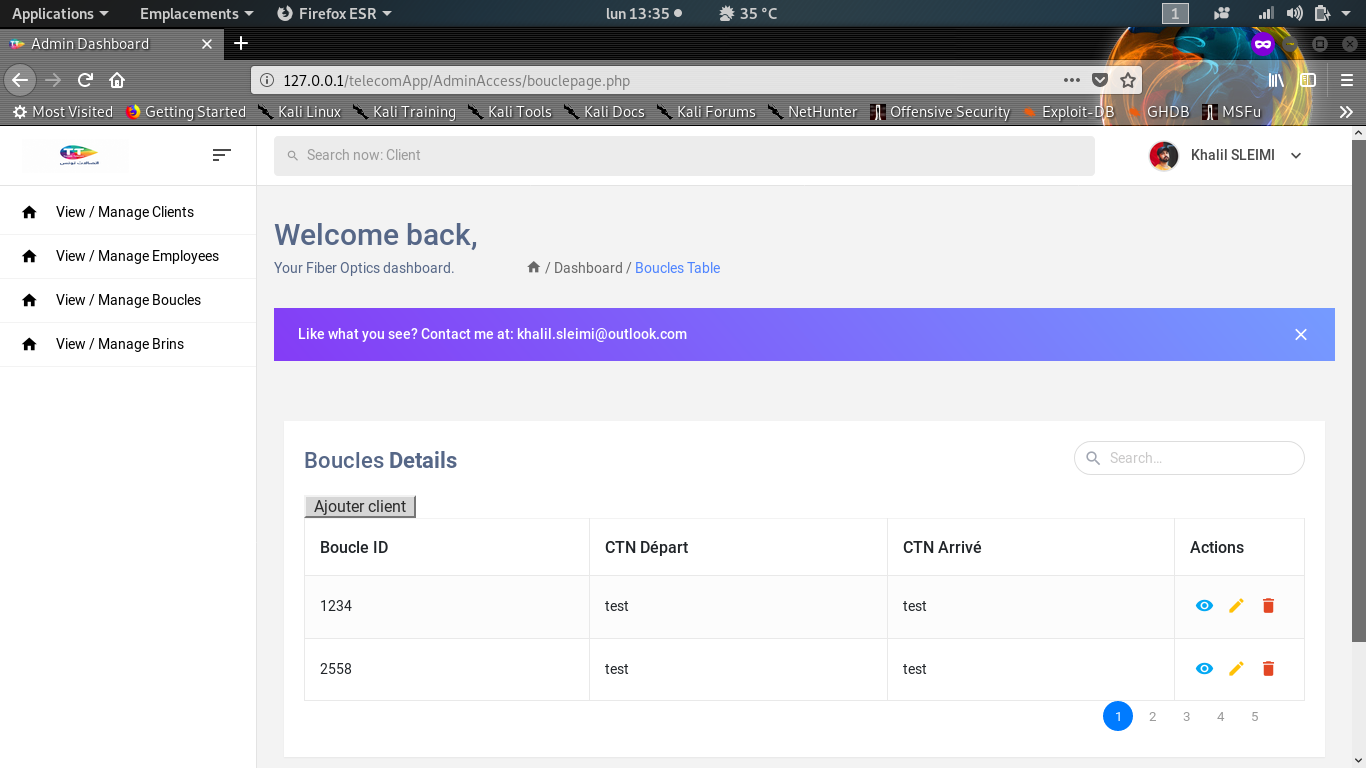
\includegraphics[width=\linewidth]{AdminBouclesTableau}
%   \caption[AdminBrinsTable]{Brins}%\index{Goku il-king}}%
%   \label{fig:AdminBrinsTable}
% \end{figure}

And in this figure is a view of how the pop up for adding and modifying Lignes - Clients is like
\begin{figure}[ht!] % supposedly places it here ...
  \centering
  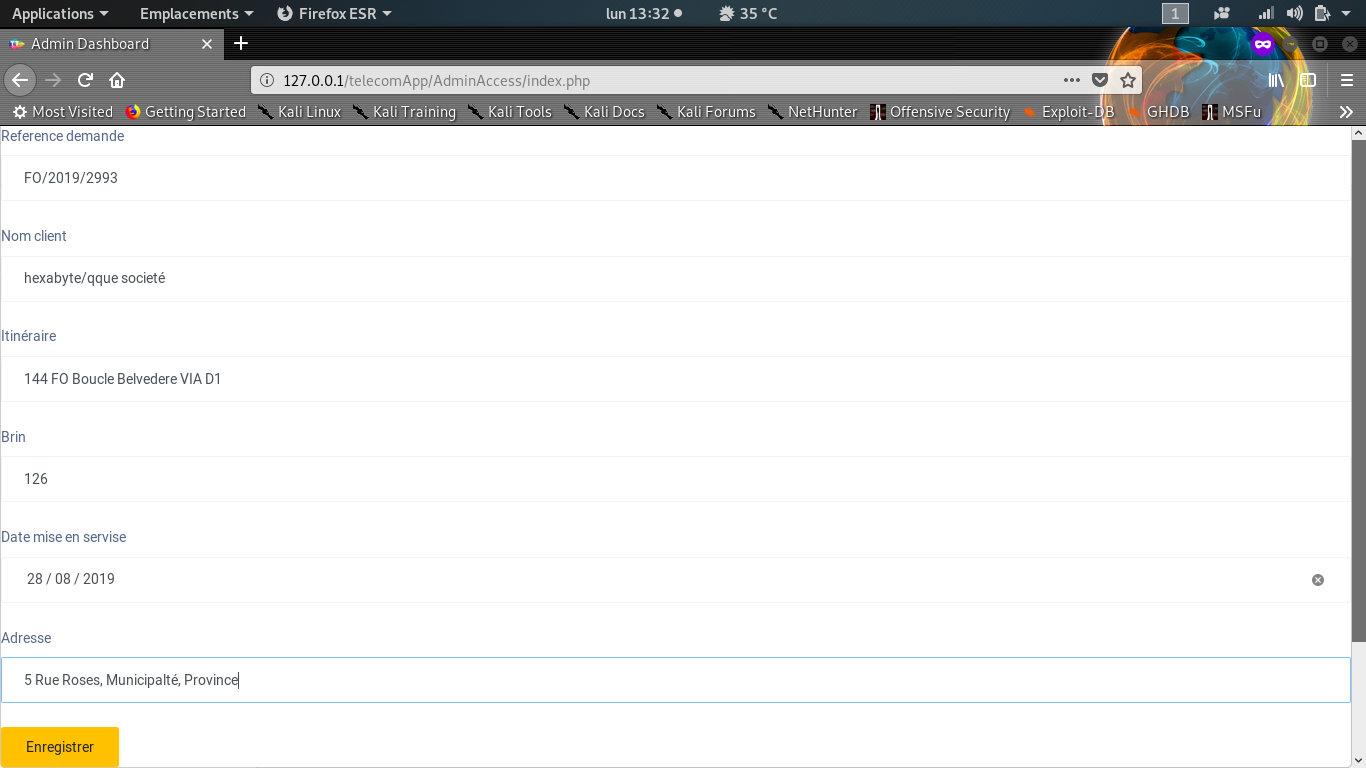
\includegraphics[width=\linewidth]{Popup}
  \caption[Client Pop Up]{Pop Up}%\index{Goku il-king}}%
  \label{fig:Popup}
\end{figure}

    \chapter{Conclusions} %Results \& Discussion
\label{chap:conc}
\textbf{Should include a reiteration of the experiments, and their outcome.  Together with a description (discussion).  Preamble should include a reminder of the aims and objectives together with a list of experiments to achieve these.  Should include many charts and other visualization with appropriate descriptions}.  

\Blindtext

\section{An Example of a Table Spanning Multiple Pages}

The following is an example of a table (Table~\ref{tab:full_dude_results}) spanning multiple pages.

\newcolumntype{P}[1]{>{\centering\arraybackslash}p{#1}}
\begin{center}
	\begingroup
	\renewcommand\arraystretch{0.66} % only applicable to this table because of group
	\begin{footnotesize}
		\begin{longtable}{lrrrrrrrr}
			\caption{Performance of Ligity in HTS mode against the Ligity-compatible DUD-E targets. The mean (and standard deviation in parentheses) values of ROC AUC using Tanimoto is 0.622 ($\pm 0.132$), while for Tversky it is 0.671 ($\pm 0.142$); the mean EF\textsubscript{1\%} using Tanimoto is 5.648 ($\pm 8.668$), while for EF\textsubscript{1\%} using Tversky it is 9.047 ($\pm 12.713$).} 
			\label{tab:full_dude_results} 
			\\ 
			\toprule 
			\multicolumn{1}{l}{\textbf{Target}}
			& \multicolumn{1}{P{1cm}}{\textbf{No.\ of Actives}}
			& \multicolumn{1}{P{1cm}}{\textbf{No.\ of Decoys}} 
			& \multicolumn{1}{P{1.25cm}}{\textbf{ROC AUC Tanimoto}} 
			& \multicolumn{1}{P{1.25cm}}{\textbf{ROC AUC Tversky}} 
			& \multicolumn{1}{P{1.25cm}}{\textbf{BEDROC Tanimoto}} 
			& \multicolumn{1}{P{1.25cm}}{\textbf{BEDROC Tversky}} 
			& \multicolumn{1}{P{1.25cm}}{\textbf{EF\textsubscript{1\%} Tanimoto}} 
			& \multicolumn{1}{P{1.5cm}}{\textbf{EF\textsubscript{1\%} Tversky}}\\	
			\midrule
			\endfirsthead
			\midrule
			\multicolumn{1}{l}{\textbf{Target}}
			& \multicolumn{1}{P{1cm}}{\textbf{No.\ of Actives}}
			& \multicolumn{1}{P{1cm}}{\textbf{No.\ of Decoys}} 
			& \multicolumn{1}{P{1.25cm}}{\textbf{ROC AUC Tanimoto}} 
			& \multicolumn{1}{P{1.25cm}}{\textbf{ROC AUC Tversky}}
			& \multicolumn{1}{P{1.25cm}}{\textbf{BEDROC Tanimoto}} 
			& \multicolumn{1}{P{1.25cm}}{\textbf{BEDROC Tversky}} 
			& \multicolumn{1}{P{1.25cm}}{\textbf{EF\textsubscript{1\%} Tanimoto}} 
			& \multicolumn{1}{P{1.25cm}}{\textbf{EF\textsubscript{1\%} Tversky}}\\	
			\midrule	
			\endhead
			\midrule	
			\multicolumn{7}{r@{}}{(continued\ldots)}\\
			\endfoot
			\endlastfoot
			ABL1   & 182   & 10,750   & 0.563   & 0.473   & 0.077   & 0.077   & 1.653   & 2.204  \\
			ACE    & 281   & 16,877   & 0.787   & 0.787   & 0.336   & 0.401   & 12.425  & 19.525 \\
			ACES   & 453   & 26,242   & 0.634   & 0.645   & 0.077   & 0.155   & 1.766   & 5.518  \\
			ADA    & 93    & 5,450    & 0.724   & 0.660   & 0.149   & 0.147   & 3.251   & 3.251  \\
			ADA17  & 532   & 35,898   & 0.638   & 0.728   & 0.103   & 0.283   & 1.317   & 9.030  \\
			ADRB1  & 247   & 15,850   & 0.523   & 0.647   & 0.065   & 0.129   & 1.619   & 5.262  \\
			ADRB2  & 231   & 14,999   & 0.523   & 0.589   & 0.052   & 0.040   & 1.735   & 0.000  \\
			AKT1   & 293   & 16,450   & 0.386   & 0.548   & 0.039   & 0.107   & 2.737   & 3.080  \\
			AKT2   & 117   & 6,900    & 0.511   & 0.685   & 0.140   & 0.194   & 8.568   & 8.568  \\
			ALDR   & 159   & 8,988    & 0.574   & 0.610   & 0.202   & 0.172   & 10.747  & 6.322  \\
			AMPC   & 48    & 2,845    & 0.521   & 0.541   & 0.049   & 0.023   & 0.000   & 0.000  \\
			ANDR   & 269   & 14,349   & 0.722   & 0.742   & 0.194   & 0.354   & 4.839   & 24.938 \\
			AOFB   & 121   & 6,875    & 0.422   & 0.464   & 0.045   & 0.027   & 1.652   & 0.000  \\
			BACE1  & 283   & 18,100   & 0.441   & 0.775   & 0.017   & 0.310   & 0.000   & 13.062 \\
			BRAF   & 152   & 9,950    & 0.612   & 0.639   & 0.208   & 0.165   & 12.502  & 5.264  \\
			CASP3  & 199   & 10,694   & 0.600   & 0.734   & 0.068   & 0.258   & 0.502   & 7.031  \\
			CDK2   & 474   & 27,838   & 0.467   & 0.507   & 0.021   & 0.048   & 0.000   & 1.055  \\
			COMT   & 41    & 3,846    & 0.789   & 0.889   & 0.338   & 0.665   & 19.447  & 58.341 \\
			CP2C9  & 120   & 7,449    & 0.518   & 0.634   & 0.058   & 0.186   & 1.660   & 8.299  \\
			CP3A4  & 170   & 11,787   & 0.450   & 0.493   & 0.022   & 0.057   & 0.000   & 2.345  \\
			CSF1R  & 166   & 12,149   & 0.526   & 0.542   & 0.136   & 0.152   & 6.031   & 7.238  \\
			CXCR4  & 40    & 3,405    & 0.575   & 0.722   & 0.217   & 0.134   & 12.665  & 0.000  \\
			DEF    & 102   & 5,699    & 0.732   & 0.833   & 0.212   & 0.379   & 10.786  & 15.689 \\
			DHI1   & 330   & 19,348   & 0.481   & 0.595   & 0.089   & 0.062   & 2.422   & 1.211  \\
			DPP4   & 533   & 40,941   & 0.586   & 0.591   & 0.154   & 0.157   & 4.312   & 3.937  \\
			DRD3   & 480   & 34,048   & 0.484   & 0.441   & 0.043   & 0.046   & 1.251   & 0.626  \\
			DYR    & 231   & 17,196   & 0.694   & 0.758   & 0.210   & 0.230   & 6.504   & 7.371  \\
			EGFR   & 542   & 35,047   & 0.593   & 0.491   & 0.054   & 0.037   & 0.922   & 0.000  \\
			ESR1   & 383   & 20,683   & 0.838   & 0.861   & 0.527   & 0.594   & 31.281  & 39.101 \\
			ESR2   & 367   & 20,199   & 0.844   & 0.870   & 0.563   & 0.644   & 20.130  & 32.644 \\
			FA10   & 537   & 28,324   & 0.564   & 0.674   & 0.058   & 0.118   & 0.930   & 2.232  \\
			FA7    & 114   & 6,249    & 0.762   & 0.859   & 0.210   & 0.332   & 6.105   & 8.721  \\
			FABP4  & 47    & 2,749    & 0.786   & 0.744   & 0.191   & 0.276   & 0.000   & 10.623 \\
			FAK1   & 100   & 5,350    & 0.642   & 0.531   & 0.111   & 0.065   & 2.019   & 0.000  \\
			FGFR1  & 139   & 8,698    & 0.511   & 0.522   & 0.036   & 0.088   & 0.722   & 1.445  \\
			FKB1A  & 111   & 5,799    & 0.605   & 0.751   & 0.162   & 0.164   & 8.122   & 3.610  \\
			FNTA   & 592   & 51,493   & 0.411   & 0.625   & 0.012   & 0.132   & 0.000   & 4.053  \\
			FPPS   & 85    & 8,842    & 0.917   & 0.985   & 0.323   & 0.776   & 2.360   & 36.581 \\
			GCR    & 258   & 14,998   & 0.805   & 0.834   & 0.244   & 0.324   & 3.092   & 8.116  \\
			GLCM   & 54    & 3,790    & 0.667   & 0.685   & 0.182   & 0.279   & 1.873   & 11.240 \\
			GRIA2  & 158   & 11,842   & 0.662   & 0.684   & 0.248   & 0.154   & 11.392  & 5.696  \\
			GRIK1  & 101   & 6,547    & 0.656   & 0.668   & 0.203   & 0.102   & 7.978   & 1.995  \\
			HDAC2  & 185   & 10,300   & 0.676   & 0.734   & 0.187   & 0.201   & 4.318   & 4.318  \\
			HDAC8  & 170   & 10,449   & 0.640   & 0.819   & 0.120   & 0.377   & 2.946   & 8.250  \\
			HIVINT & 100   & 6,640    & 0.390   & 0.554   & 0.030   & 0.116   & 0.000   & 3.018  \\
			HIVPR  & 535   & 35,724   & 0.663   & 0.872   & 0.072   & 0.490   & 0.187   & 23.898 \\
			HIVRT  & 338   & 18,884   & 0.495   & 0.475   & 0.124   & 0.085   & 4.443   & 1.777  \\
			HMDH   & 170   & 8,750    & 0.480   & 0.906   & 0.068   & 0.652   & 2.358   & 35.963 \\
			HS90A  & 88    & 4,850    & 0.635   & 0.506   & 0.096   & 0.083   & 0.000   & 3.436  \\
			HXK4   & 92    & 4,700    & 0.662   & 0.803   & 0.206   & 0.307   & 15.192  & 9.766  \\
			IGF1R  & 148   & 9,300    & 0.502   & 0.575   & 0.057   & 0.189   & 2.037   & 14.941 \\
			INHA   & 43    & 2,300    & 0.493   & 0.575   & 0.031   & 0.045   & 0.000   & 0.000  \\
			ITAL   & 138   & 8,500    & 0.619   & 0.465   & 0.037   & 0.065   & 0.000   & 0.728  \\
			JAK2   & 107   & 6,500    & 0.472   & 0.475   & 0.073   & 0.118   & 2.807   & 6.549  \\
			KIF11  & 116   & 6,850    & 0.755   & 0.781   & 0.149   & 0.219   & 4.289   & 2.574  \\
			KIT    & 166   & 10,449   & 0.463   & 0.437   & 0.045   & 0.030   & 0.000   & 0.000  \\
			KITH   & 57    & 2,850    & 0.649   & 0.838   & 0.228   & 0.709   & 14.069  & 47.483 \\
			KPCB   & 135   & 8,699    & 0.753   & 0.813   & 0.220   & 0.338   & 8.923   & 12.641 \\
			LCK    & 419   & 27,391   & 0.471   & 0.437   & 0.031   & 0.043   & 0.000   & 1.910  \\
			LKHA4  & 171   & 9,448    & 0.718   & 0.694   & 0.238   & 0.150   & 8.203   & 1.758  \\
			MAPK2  & 101   & 6,148    & 0.660   & 0.670   & 0.174   & 0.199   & 5.988   & 3.992  \\
			MCR    & 94    & 5,149    & 0.816   & 0.888   & 0.215   & 0.454   & 6.436   & 19.307 \\
			MET    & 166   & 11,249   & 0.566   & 0.531   & 0.130   & 0.065   & 6.032   & 0.603  \\
			MK01   & 79    & 4,550    & 0.518   & 0.602   & 0.121   & 0.206   & 5.095   & 3.821  \\
			MK10   & 104   & 6,600    & 0.488   & 0.489   & 0.020   & 0.031   & 0.962   & 0.962  \\
			MK14   & 578   & 35,847   & 0.511   & 0.589   & 0.040   & 0.064   & 0.173   & 0.519  \\
			MMP13  & 572   & 37,199   & 0.648   & 0.753   & 0.134   & 0.268   & 2.446   & 9.957  \\
			MP2K1  & 121   & 8,146    & 0.669   & 0.569   & 0.187   & 0.058   & 3.293   & 0.823  \\
			NOS1   & 98    & 8,028    & 0.483   & 0.451   & 0.109   & 0.041   & 3.071   & 0.000  \\
			NRAM   & 98    & 6,200    & 0.853   & 0.859   & 0.342   & 0.290   & 11.221  & 3.060  \\
			PA2GA  & 99    & 5,150    & 0.793   & 0.756   & 0.225   & 0.153   & 1.020   & 3.059  \\
			PARP1  & 508   & 30,029   & 0.635   & 0.692   & 0.215   & 0.231   & 11.234  & 7.884  \\
			PGH1   & 195   & 10,798   & 0.645   & 0.637   & 0.077   & 0.100   & 0.000   & 2.050  \\
			PGH2   & 435   & 23,139   & 0.716   & 0.780   & 0.166   & 0.291   & 3.444   & 9.874  \\
			PLK1   & 107   & 6,800    & 0.658   & 0.531   & 0.123   & 0.048   & 1.871   & 0.000  \\
			PNPH   & 103   & 6,946    & 0.575   & 0.578   & 0.161   & 0.181   & 4.888   & 8.799  \\
			PPARA  & 373   & 19,399   & 0.783   & 0.778   & 0.262   & 0.280   & 6.693   & 7.764  \\
			PPARD  & 240   & 12,250   & 0.547   & 0.544   & 0.078   & 0.098   & 1.665   & 2.498  \\
			PPARG  & 484   & 25,299   & 0.515   & 0.605   & 0.055   & 0.118   & 0.619   & 4.955  \\
			PRGR   & 293   & 15,648   & 0.740   & 0.793   & 0.142   & 0.318   & 2.053   & 14.714 \\
			PTN1   & 130   & 7,249    & 0.398   & 0.538   & 0.055   & 0.090   & 0.000   & 3.068  \\
			PUR2   & 50    & 2,700    & 0.851   & 0.837   & 0.281   & 0.255   & 7.857   & 1.964  \\
			PYGM   & 77    & 3,944    & 0.403   & 0.492   & 0.016   & 0.137   & 0.000   & 3.917  \\
			PYRD   & 111   & 6,449    & 0.682   & 0.710   & 0.462   & 0.413   & 34.027  & 16.118 \\
			RENI   & 104   & 6,956    & 0.720   & 0.789   & 0.043   & 0.138   & 0.000   & 0.000  \\
			ROCK1  & 100   & 6,300    & 0.347   & 0.449   & 0.020   & 0.084   & 1.000   & 4.000  \\
			RXRA   & 131   & 6,950    & 0.788   & 0.900   & 0.219   & 0.596   & 6.091   & 27.407 \\
			SAHH   & 63    & 3,450    & 0.874   & 0.852   & 0.598   & 0.542   & 35.050  & 27.084 \\
			SRC    & 524   & 34,500   & 0.565   & 0.477   & 0.065   & 0.050   & 0.382   & 0.573  \\
			TGFR1  & 133   & 8,499    & 0.609   & 0.639   & 0.147   & 0.154   & 10.565  & 4.528  \\
			THB    & 103   & 7,450    & 0.794   & 0.762   & 0.238   & 0.150   & 10.614  & 0.965  \\
			THRB   & 461   & 27,000   & 0.605   & 0.706   & 0.063   & 0.166   & 2.166   & 5.632  \\
			TRY1   & 449   & 25,975   & 0.711   & 0.815   & 0.147   & 0.280   & 2.898   & 6.688  \\
			TRYB1  & 148   & 7,650    & 0.670   & 0.670   & 0.153   & 0.132   & 3.378   & 3.378  \\
			TYSY   & 109   & 6,745    & 0.594   & 0.725   & 0.071   & 0.226   & 0.911   & 5.468  \\
			UROK   & 162   & 9,850    & 0.525   & 0.650   & 0.036   & 0.120   & 0.000   & 1.854  \\
			VGFR2  & 409   & 24,948   & 0.632   & 0.578   & 0.083   & 0.093   & 1.465   & 1.465  \\
			WEE1   & 102   & 6,150    & 0.934   & 0.929   & 0.789   & 0.797   & 59.348  & 61.294 \\
			XIAP   & 100   & 5,150    & 0.752   & 0.974   & 0.190   & 0.897   & 8.077   & 51.490 \\
			\bottomrule
			
		\end{longtable}
	\end{footnotesize}
	\endgroup
\end{center}

\section{Some Other Section}
\Blindtext

\section{A Landscape Table Example}
Next is an example of a wide table on a landscape oriented paper.
	
\begin{landscape}
	\pagestyle{empty} %% only if you want to remove silly headers on the side
	\begin{tabular}{rrrrrrrrrrrrrrr} \toprule
		{$m$} & {$x$} & {$y$} & {$z$} & {$a$} & {$A_m$} & {$B$} & {$C$} & {$x$} & {$y$} & {$z$} & {$a$} & {$A_m$} & {$B$} & {$C$} \\ \midrule
		1  & 16.128 & +8.872 & 16.128 & 1.402 & 1.373 & -146.6 & -137.6 & 16.128 & +8.872 & 16.128 & 1.402 & 1.373 & -146.6 & -137.6\\
		2  & 3.442  & -2.509 & 3.442  & 0.299 & 0.343 & 133.2  & 152.4 & 3.442  & -2.509 & 3.442  & 0.299 & 0.343 & 133.2  & 152.4 \\
		3  & 1.826  & -0.363 & 1.826  & 0.159 & 0.119 & 168.5  & -161.1 & 1.826  & -0.363 & 1.826  & 0.159 & 0.119 & 168.5  & -161.1 \\
		4  & 0.993  & -0.429 & 0.993  & 0.086 & 0.08  & 25.6   & 90 & 1.826  & -0.363 & 1.826  & 0.159 & 0.119 & 168.5  & -161.1    \\ \midrule
		5  & 1.29   & +0.099 & 1.29   & 0.112 & 0.097 & -175.6 & -114.7 & 1.826  & -0.363 & 1.826  & 0.159 & 0.119 & 168.5  & -161.1\\
		6  & 0.483  & -0.183 & 0.483  & 0.042 & 0.063 & 22.3   & 122.5 & 1.826  & -0.363 & 1.826  & 0.159 & 0.119 & 168.5  & -161.1 \\
		7  & 0.766  & -0.475 & 0.766  & 0.067 & 0.039 & 141.6  & -122 & 1.826  & -0.363 & 1.826  & 0.159 & 0.119 & 168.5  & -161.1  \\
		8  & 0.624  & +0.365 & 0.624  & 0.054 & 0.04  & -35.7  & 90  & 1.826  & -0.363 & 1.826  & 0.159 & 0.119 & 168.5  & -161.1   \\ \midrule
		9  & 0.641  & -0.466 & 0.641  & 0.056 & 0.045 & 133.3  & -106.3 & 1.826  & -0.363 & 1.826  & 0.159 & 0.119 & 168.5  & -161.1\\
		10 & 0.45   & +0.421 & 0.45   & 0.039 & 0.034 & -69.4  & 110.9  & 1.826  & -0.363 & 1.826  & 0.159 & 0.119 & 168.5  & -161.1\\
		11 & 0.598  & -0.597 & 0.598  & 0.052 & 0.025 & 92.3   & -109.3 & 1.826  & -0.363 & 1.826  & 0.159 & 0.119 & 168.5  & -161.1\\ \bottomrule
	\end{tabular}
\end{landscape}

\section{Summary}
\blindtext\enlargethispage{\baselineskip} % so you do not get a single line in another page
    \chapter{Evaluation}

\textbf{In an ideal world, you should have two kind of evaluations.  The first is against some ground truth (perhaps a random model?).  The second kind of evaluation is against other people's work (accuracy, speed, etc.).  Any dimension which is of interest, should be evaluated.  Evaluation should be statistically sound. }

\Blindtext

\section{Summary}
\blindtext
    \chapter{Conclusions}
\textbf{This section should have a summary of the whole project.  The original aims and objective and whether these have been met should be discussed. It should include a section with a critique and a list of limitations of your proposed solutions.  Future work should be described, and this should not be marginal or silly (e.g.\ add machine learning models).  It is always good to end on a positive note (i.e.\ `Final Remarks').}

\section{Achieved Aims and Objectives}
\blindtext

\section{Critique and Limitations}
\blindtext

\section{Future Work}
\blindtext

\section{Final Remarks}
\blindtext

    \appendix
        \chapter{Media Content}

If the dissertation has a DVD or pendrive attached to it, you will need a section which explains what is on the media (structure, files, data, etc.).  This could be a table with filename and description.

\blindtext
     % these are just test names as I didn't know what you'd want
        \chapter{Installation Instructions}
\blindtext
    
        \chapter{User Manual}
\Blindtext
 

{\backmatter
    % Bibliography
    \if@openright\cleardoublepage\else\clearpage\fi
    \bibliographystyle{um-plainnat} %% specific plainnat does not show url for articles
    {\footnotesize\bibliography{chap1/introduction_biblio,chap2/background_and_lit_overview_biblio}}
	\printindex
}

\end{document}

%%% The End %%%